\documentclass[12pt,a4paper]{article}

\usepackage[T1]{fontenc}
\usepackage[utf8]{inputenc}
\usepackage[margin=2.5cm]{geometry}
\usepackage{graphicx}
\usepackage[hidelinks]{hyperref}
\usepackage{fancyhdr}
\usepackage{lastpage}
\usepackage{appendix}
\usepackage{amsmath}
\usepackage{color}
\usepackage{palatino}
\usepackage{changepage}
\usepackage{subcaption}
\usepackage{enumitem}
\usepackage{csquotes}
\usepackage{verbatim}
\usepackage[cache=false]{minted}
\usepackage[ruled,vlined]{algorithm2e}

\usemintedstyle{fruity}

\title{Community detection in networks}
\author{Carlos Requena López}

%% Fancy layout
\pagestyle{fancy}
\lhead{INFO-F521}
\chead{}
\rhead{}
\lfoot{}
\cfoot{}
\rfoot{Page \thepage\ of \pageref{LastPage}}
\renewcommand{\headrulewidth}{0.4pt}
\renewcommand{\footrulewidth}{0.4pt}


%%% --- %%% --- DOCUMENT START --- %%% --- %%%
\begin{document}
\thispagestyle{fancy}
\maketitle
\thispagestyle{fancy}

\section{Introduction}

The topic of this assignment is community detection in networks by
means of hierarchical clustering. Informally, network communities can
be seen as dense (highly connected) subgraphs that are connected
between each other sparsely, only by few arcs or edges.

Hierarchical clustering (HC) refers to the technique of grouping
together elements that share some sort of similarity and separating
those that do not. HC can be \emph{divisive}, where elements start in
one cluster and are removed gradually or \emph{agglomerative}, where
every unit is its own cluster and are merged step by step. Only
\emph{agglomerative} clustering will be considered in this assignment:
in particular single-linkage and complete-linkage clustering.

\section{Analysis and expectations}

\subsection{Measure of similarity}

Let $ G = (V, E) $ be a simple, unweighted, undirected graph. Let $A$
be the adjacency matrix of $G$, defined as follows:

\[
  A_{ij} =
  \begin{cases}
    1 & \quad \text{if } (i,j) \in E\\
    0 & \quad \text{otherwise }
  \end{cases}
\]

We will use this adjacency matrix as the only source of information to
determine the similarity between vertices in the graph, but there
could be plenty of other sources depending on the application
domain. For example, when analysing text files, the similarity measure
could be the amount of equal significant words each one contains, or
in the case of aminoacids, the number of times it appears on protein
$p$ at location $l$.

Here, however, we compute the mean and variance between the rows of
the adjacency matrix as follows (if $A$ was not symmetric and $G$
undirected, it would have to be computed for rows \emph{and} columns):

$$ \mu_i = \frac{1}{n} \sum_{j=1}^{n} A_{ij} $$

$$ \sigma^2 = \frac{1}{n} \sum_{j=1}^{n} (A_{ij} - \mu_i)^2 $$

The similarity measure in this case is the Pearson product-moment
correlation coefficient:

$$ x_{ij} = \frac{\frac{1}{n}\sum_{k=1}^{n}(A_{ik} -
  \mu_i)(A_{jk}-\mu_j)}{\sigma_i\sigma_j} $$

All diagonal elements are excluded from these calculations
\cite[p.~369]{socionetwork}. The value $x_{ij}$ can range from -1 to
1, and it gives a measure of how structurally similar two vertices
are.

\subsection{Hierarchical clustering}

Once the similarity measures are developed, they serve as a base to
implement agglomerative HC. By observing the set of partitions (the
number of partitions is the number of elements at step 0), we can
define the function to maximise when deciding which two partitions to
merge. This is repeated until there is only one partition (containing
all the elements) left.

Algorithms for HC do not require the size of the partitions of the
number of partitions to be specified. Obviously, the output of the
program - a set containing all vertices - is not really meaningful;
that is why the process is captured in a data structure called
\emph{dendogram}

\subsubsection{Single-linkage clustering}

The main formula behind the concept of complete linkage is:

$$ \mathrm{max}\{x_{i,j} : i \in P_a, j \in P_b\} $$

where ${P_a}$ and $P_b$ are two partitions of $V$.

\subsubsection{Complete-linkage clustering}

In contrast to the complete linkage method, single linkage will look
the least similar vertices among pairwise observations:

$$ \mathrm{min}\{x_{i,j} : i \in P_a, j \in P_b\} $$

In both cases, those are the functions to satifisfy when merging new
partitions.


For example, for the simple graph given in
fig. \ref{fig:simple_graph}, the means, variances and similarity
measures are given in table

\begin{figure}[ht!]
  \centering
  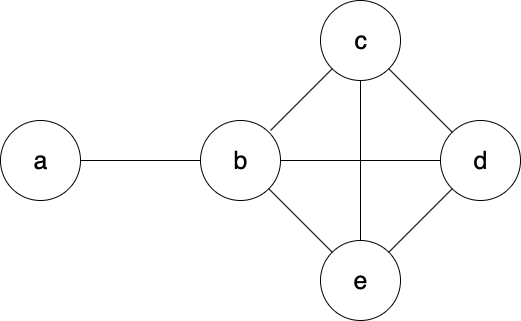
\includegraphics[width=0.6\textwidth]{img/simple_graph.png}
  \caption{Simple graph with 5 vertices}
  \label{fig:simple_graph}
\end{figure}

Let's answer the questions formulated in the statement:

\begin{description}
\item[Pseudocode of single linkage and complete linkage algorithms] \hfill
  \\
  The pseudocodes for basic single linkage and complete linkage
  algorithms are given in \ref{slink} and \ref{clink}
  \begin{algorithm}[h]
    \SetAlgoLined
    \KwIn{An undirected connected graph G}
    \KwOut{The tree of clusters}

    \nl Compute the proximity (similarity) matrix X for the given G.\;
    \nl Place every vertex in its own set.\;
    \nl Find the two most similar sets and merge them.\;
    \nl Remove the entry in X and update it by choosing the highest
    values possible.\;
    \nl Append merge information to tree to keep the history of events.\;
    \nl \While{X \textrm{has shape} > 1x1}{
      \nl Repeat lines 3 through 5\;
    }
    \caption{\bf SLOW_S-LINK}
    \label{slink}
  \end{algorithm}

  \begin{algorithm}[h]
    \SetAlgoLined
    \KwIn{An undirected connected graph G}
    \KwOut{The tree of clusters}

    \nl Compute the proximity (similarity) matrix X for the given G.\;
    \nl Place every vertex in its own set.\;
    \nl Find the two least similar sets and merge them.\;
    \nl Remove the entry in X and update it by choosing the lowest
    values possible.\;
    \nl Append merge information to tree to keep the history of events.\;
    \nl \While{X \textrm{has shape} > 1x1}{
      \nl Repeat lines 3 through 5\;
    }
    \caption{\bf SLOW_C-LINK}
    \label{clink}
  \end{algorithm}

\item[Computational complexity] \hfill \\

  For both cases, the complexity of the algorithm is
  $\mathcal{O}(n^3)$: computing the similarity matrix (or distance
  information) takes $\mathcal{O}(nm)$ \cite{newman}, where $n$ is the
  number of vertices and $m$ is the number of edges. We need to check
  the minimum element in an array of size $n^2$, so, by the adversary
  argument, this takes $\mathcal{O}(n^2)$, and this check has to be
  done a maximum of $n$ times. Therefore, the naive upper bound is
  $\mathcal{O}(n^3)$.

\item[Difference between single link and complete link.] \hfill \\
  On the one hand, single-linkage combines two clusters or partitions
  that contain the closest (or most similar) pair of elements that are
  not yet merged into a single cluster. It favours

  On the other hand, complete linkage

  A third approach not discussed here, \emph{average linkage}, does
  not consider a single vertex (the one with lowest or highest) per
  partition to match into another partition. Instead, it computes an
  average of similarities among the members of that partition to
  determine if they are similar (or distant) enough to be merged with
  another partition.

\item[Optimality of solution at each step] \hfill \\



\item[What happens in the case of a tie?]  \hfill \\

  Several approaches exist to deal with the non-uniqueness problem of
  similarities in the data set \cite{nonunique}:

  \begin{itemize}
  \item Arbitrarily choosing between the elements in the tie.
  \item Deterministically choosing between the elements in the tie
    (the element with smaller index for example).
  \item Merge all tied elements at the same time.
  \end{itemize}



\end{description}



\section{Implementation}

The graph $ G $ is given as an adjacency matrix, which is parsed

\section{Results}

\section{Conclusion}

% \begin{figure}[ht!]
%   \centering
%   \includegraphics[width=1\textwidth]{some_graphic.png}
%   \caption{}
%   \label{fig:fig1}
% \end{figure}

\bibliographystyle{ieeetr}
\bibliography{main}
\nocite{*}

\appendix
\section{Appendix - code listing}

\inputminted{python}{../src/main.py}

% \begin{minted}{minted}
% \end{minted}


\end{document}
